\section{Preliminaries}\label{sec:preliminiary}

\eray{}{-comment: It would be mention the time scales in the network somewhere in the beginning, e.g., with a simple figure for slot time, epoch, era, and mention how long they are. I couldn't find these time scales easily when I was searching for them.-}

\handan{}{should we have this section before properties section? If prop section comes after this section we should remove some descriptions of entities in the properties section e.g., validator, fisherman}
\eray{}{-comment: I agree. I think it may help the reader understand the properties better after reading the design.-}
\syed{}{+1}
\syed{}{We need an intro here before jumping into the figures; the following is inspired by the intro in the original white paper}
Polkadot network consists of a large number of validatable, globally-coherent dynamic “parallelised” data-structures called  <i>parachains</it> and the bedrock upon which those parachains are interacting, are known as <it>the relay chains</it>. Figure \ref{fig:roles} shows these subcomponents alongside the sub-actors of the system which are in play to deliver the Polkadot scalable heterogeneous multi-chain system.

\begin{figure}[h]
	\centering
	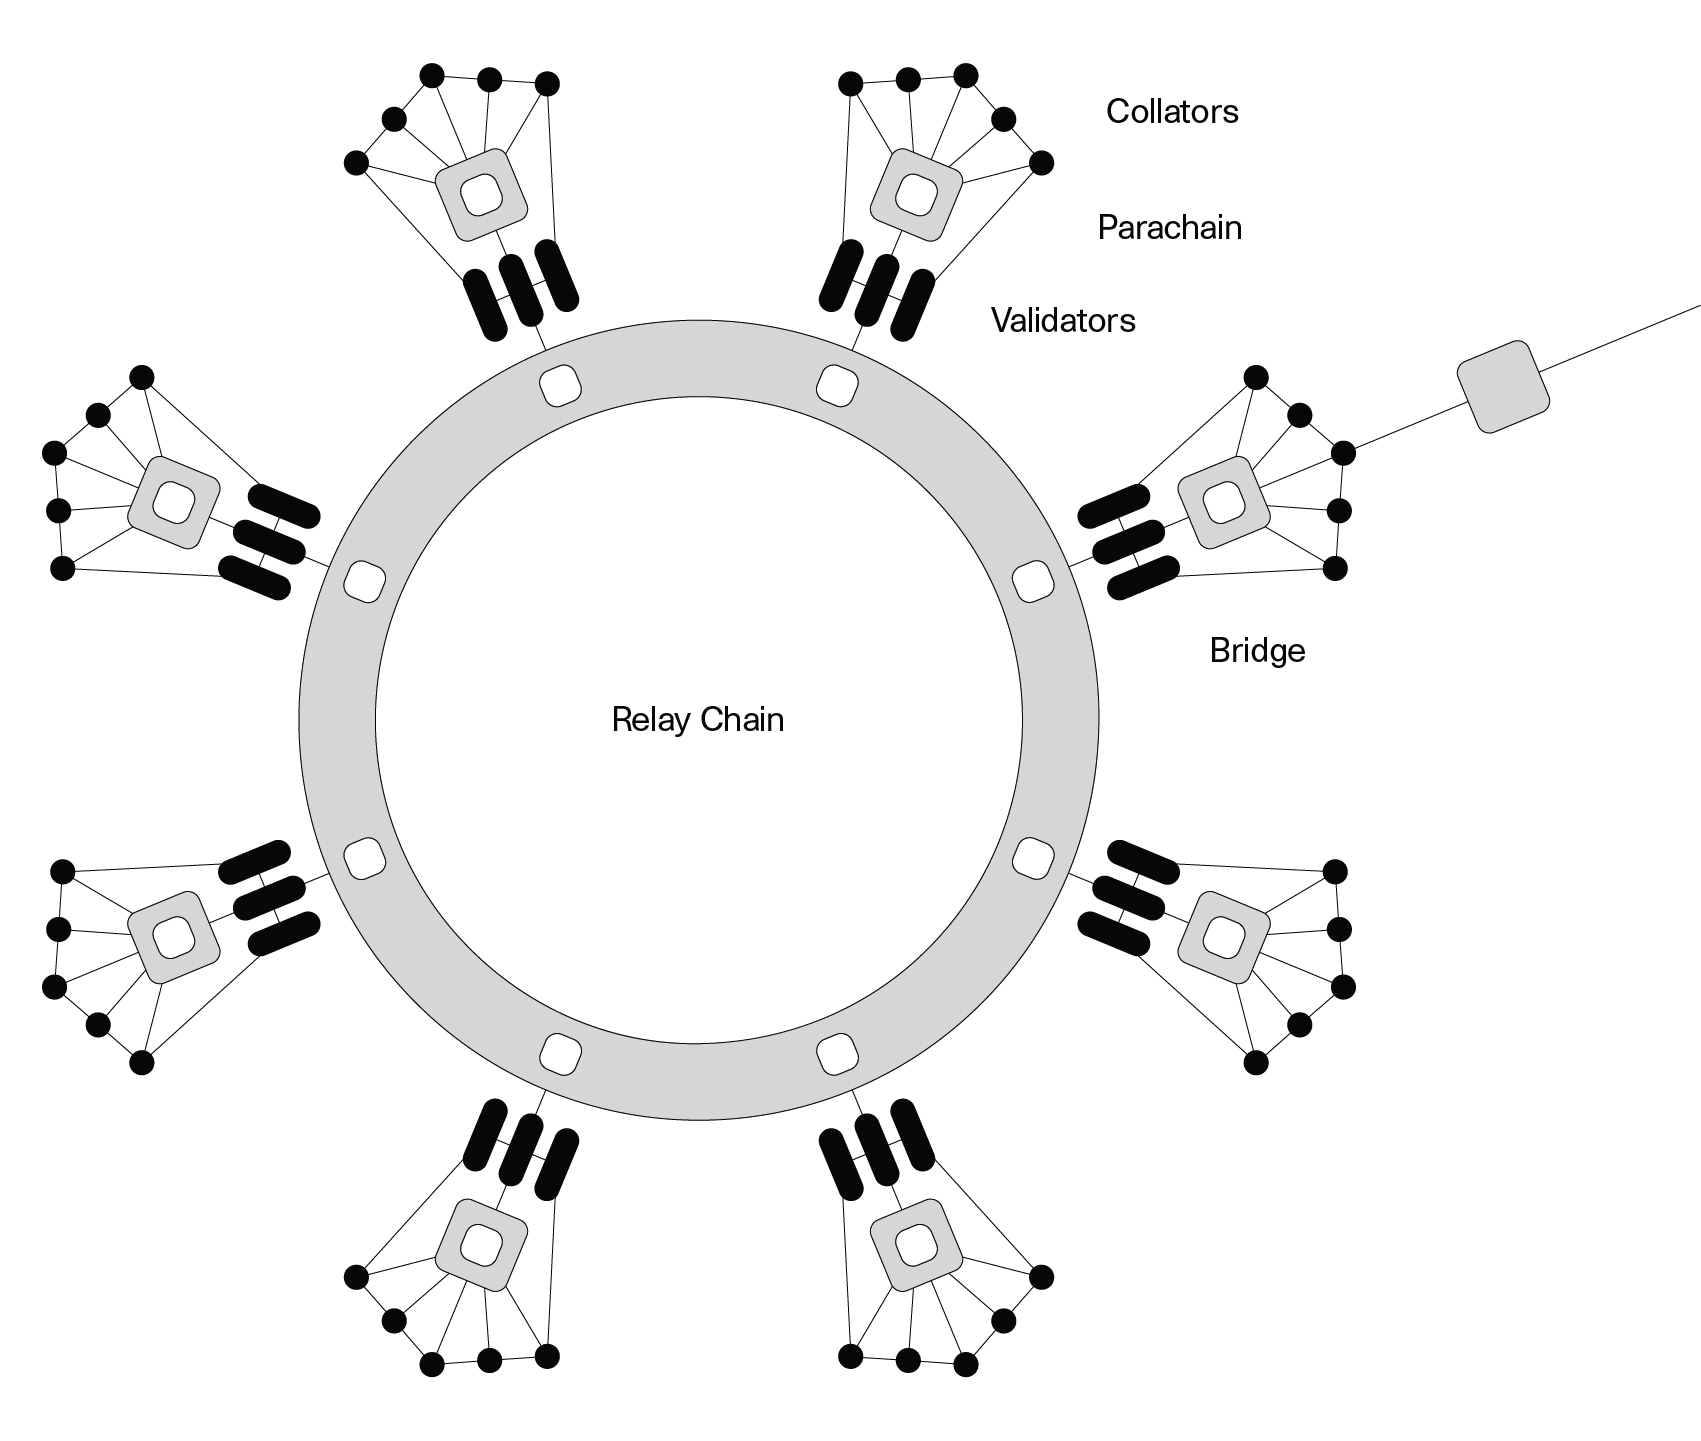
\includegraphics[width=.7\textwidth]{images/Network@2x.png}
	\caption{Polkadot network structure showing relay chain and parachain and including the roles collator, validator (Image credit: Ignasio Albero)}
	\label{fig:roles}
\end{figure}
\subsection{Structural elements of Polkadot}
\syed{Next}{In this section}, we review the structural elements and \syed{roles}{different roles defined in the Polkadot protocol and, as} shown in Figure~\ref{fig:roles}\syed{, that are defined for the Polkadot protocols}{-remove-}.

\syed{}{perhaps we should use more technical language in this section. I'll try to do so in my review.}

\paragraph{Chain} (or a blockchain) broadly refers to a state machine which possibly replicated in a decentralized environment. By a block we refer to a recorded list of transactions which have been applied to change the state of a chain.

\paragraph{Parachains:} \syed{Multiptle heterogeneous blockchains run in parallel in Polkadot.}{I feel this definition is barely helpufl}

\paragraph{Relay Chain:} \syed{This is}{is} \syed{a}{the Polkadot} central \syed{chain}{state machine} \syed{in Polkadot.}{-remove-} which keeps references to \syed{all canonical parachain blocks}{the current states of all parachains and to the cross parachain transactions}. \syed{and t}{T}hus \syed{}{the relay chain} works as a single source of truth across \syed{parachains}{Polkadot network}.
\syed{It also keeps references of all cross-parachain messages}{-remove- mentioned above as cross parachain transaction, what is a message otherwise? we need to define it first}.

\subsection{Roles}

\syed{}{Nodes which run Polkadot network assume diffierent roles to ensure the properties introduced in Section \ref{sec:properties}. In the following, we intorduce these roles and their functions.}

\syed{}{I'm looking at the definition of these roles in the original paper and in many case they look more comprehensive than what we have here. Perhaps, we could incorporate more of the original white paper here.}
  
\paragraph{Validators:} A fixed set of actors called validators are responsible to \syed{maintain}{what is maintain? shouldn't we be specific} the relay chain
and keep its consensus, and by extension, maintain the consensus of all the parachains.
\syed{In addition}{Moreover}, at regular intervals validators are divided into random disjoint subsets
that are each assigned to a particular parachain.
Each of these validator subsets ensures the validity and availability of its parachain's blocks.
Validators receive regular remunerations in DOTs,
and are likewise heavily \syed{staked}{define} and prone to \syed{slashing}{define} in case of offenses. \syed{}{in contrast see the comprehensive definition in the white paper page 4}

\paragraph{Nominators:} The role of validator is \eray{permissionless}{-comment: I do not understand what is meant by permissonless.-}
 (like all roles in Polkadot),
but the number of slots for validators is limited. Hence, validators must be elected by the community.
In particular, any DOT holder may assume the role of a \emph{nominator}, lock some stake, and publish a list
of trusted validator candidates. Candidates with the most nominators' support get elected,
and nominators share the economic rewards, or slashes, of their supported validators.
Having nominators allows for an unlimited amount of actors and DOTs to participate in the security of Polkadot.

\paragraph{Collators: } Every parachain has its own set of full nodes called collators.
A collator produces new blocks and sends it to the \handan{parachain-assigned validators}{why not just parachain validators?}.
It may only build on top of the parachain blocks that are referenced in the relay chain.
Collators also process outgoing and incoming cross-chain messages.

\paragraph{Fishermen:} Fishermen are staked actors that run background checks on the performance of validators.
In particular, they raise reports in case that a validator-approved parachain block is unavailable or invalid.
They are rewarded for correct reports, and slashed for bogus ones (which helps avoid report spamming).


\subsection{Adversarial Model of Polkadot}

%The adversarial assumption on collators depends on the parachain type. If the parachain is private,
%we assume that there is at least one honest collator.
%Otherwise, we assume that at least the majority of collators are honest.
\paragraph{Roles:} In general, we assume that honest parties follow the protocol while malicious ones can follow any arbitrary algorithm. We assume that three quarters of nominators' stake belong to honest ones. As a result of this assumption, more than two third of validators who are elected by nominators are honest. We do not have any limit on number of malicious fishermen since their malicious behaviours are detectable and punishable.  

\paragraph{Parachains:} We do not have any security assumption on block production mechanism of parachain. On the other hand, we assume that a significant amount of collators are honest. The security of Polkadot does not depend on any precise honest fraction of collators but it requires existence of some honest collators.

\paragraph{Keys:} We assume that malicious parties generate their keys with an arbitrary algorithm
while honest ones always generate their keys securely. 

\paragraph{Network and Communication:} All validators have their own local clock and their clocks do not rely on any central clock.
We assume that  validators and collators are in a partially synchronous network.
It means that a message sent by a validator or collator arrives at all parties in the network
at most $\D$ units of time later where $\D$ is an unknown parameter. So, we assume an eventual delivery of a message in Polkadot.
We also assume that collators and fishermen can connect to the relay chain network to submit their reports.
%TODO: Do we have authenticated channel between validators?
